%
\documentclass[Journal]{ascelike}
%
\usepackage{endfloat}
\usepackage{setspace}
\usepackage{longtable}
\usepackage{epsfig}
\usepackage{amssymb}
\usepackage{amsmath}
\usepackage{manyeqns}
\usepackage{graphicx}
%\usepackage{footnote}
%\usepackage{appendix}
\usepackage[letterpaper, top=25.4mm, bottom=10mm, left=25.4mm, right=25.4mm]{geometry}
%
\begin{document}
%
% You will need to make the title all-caps
\title{Bayesian Estimation of the multi-state Markov Model}
%
\author{Kiyoyuki Kaito%
\thanks{Associate Professor, Dr., Graduate School of Engineering, Osaka University, Suita, Osaka, Japan. \hspace{10mm}E-mail: kaito@ga.eng.osaka-u.ac.jp}, Kiyoshi Kobayashi \thanks{Professor, Dr., Dept. of Urban Management., Kyoto University, Katsura, Nishikyo-ku, Kyoto, Japan. \hspace{10mm}E-mail: kkoba@psa.mbox.media.kyoto-u.ac.jp} and Nam Lethanh \thanks{Postdoc, Dr., Institute for Construction and Infrastructure Management., Swiss Federal Institute of Technology (ETH), Zurich, Switzerland. E-mail: lethanh@ibi.baug.ethz.ch}
\ %Member, ASCE
%
}
%
\maketitle
%
\begin{abstract}
%
%This paper presents a novel approach using Bayesian methodology to estimate the Markov transition probability in Markov deterioration forecasting model used in infrastructure management system. Markovian transition probability is often estimated by employing maximum likelihood estimation approach on historical monitoring data. However, the method
In many practices of bridge asset management, life cycle costs are estimated by statistical deterioration prediction models based upon visual inspection data. In many applications, it is, however, often the case that the validity of statistical deterioration prediction models is flawed by an inadequate stock of inspection dates. In this paper, a systematic methodology is presented to provide estimates of the deterioration process for bridge managers based upon empirical judgments at early stages by experts, and whereby revisions may be made as new data are obtained through later inspections. More concretely, the Bayesian estimation methodology is presented to improve the multi-state Markov model by the Markov Chain Monte Carlo method. The paper concludes with examples of the methodology presented in this paper applied to a data set in the real field.
\end{abstract}
%
\\
\textbf{CE Database subject headings:} Bayesian estimation; Markov Chain Monte Carlo; Gibbs sampling; Statistical deterioration prediction; Asset management.

\section{Introduction}
\label{section1}
In the asset management for civil infrastructures, it is important to determine optimal intervention strategies based on the analysis of life cycle costs (LCC) \cite{Kobayashi2007a,KobayashiKiyoshi2003}. Life cycle costs are the sum of all expenses incurred to stakeholders (owners, users, and public) during the lifetime of civil infrastructures. The LCC analysis is often carried out either with minimization of discount flow method \cite{Jido2008} or minimization of annual average cost method \cite{Kobayashi2007a,Kaito2005}. One important, but subtle, feature of the LCC analysis is that it has to be dependent on the deterioration model, which is employed to predict the deterioration of civil infrastructure. The deterioration model is therefore considered as the heart of an infrastructure management system (IMS). 

To the authors's knowledge, so far in infrastructure asset management study area, researchers employ two kinds of deterioration prediction methods: 1) one targets the average deterioration of all related civil infrastructures, and 2) the other targets the concrete damage and deterioration of each infrastructure or member. For the former, a statistical method is often adopted in order to model the regularities behind deterioration processes based on an enormous amount of deterioration information. For the latter, a physical method is frequently adopted in order to directly model deterioration processes by clarifying the deterioration mechanism. In addition, when surveying the actual condition state of asset management, it is common at the outset to grasp the deterioration characteristics of the entire civil infrastructures, make decisions on intervention strategies (such as the selection of methods for preventive maintenance or posteriori maintenance), and then design concrete intervention plans for each infrastructure. In favor of statistical method in deterioration prediction, this study aims to improve the application of statistical deterioration prediction models by introducing a novel method using Bayesian estimation.

The authors have developed statistical deterioration estimation methods \cite{Kaito2002,kobayashitsuda} based on visual inspection data, conducted many empirical studies using actual data, and verified their effectiveness. However, it has been realized that in order to assure a high accuracy in deterioration prediction, it is necessary to collect several thousands of visual inspection data \cite{sugisakia,kobayashitsuda}. With regard to data amount, most infrastructure administrators face the problems of insufficient amounts of data, and it is anticipated that the insufficiency of data will hinder the practical application of a statistical method. Suffice it to say that in order to improve the applicability of statistical methods, it is essential to develop a methodology which can provide estimation results by fusing prior information, such as the experience, knowledge, and know-how of professional engineers, with a limited amount of visual inspection data, accumulate additional data, and update the estimation results constantly.%, even when visual inspection data have not yet been accumulated sufficiently.

Under this circumstance, this study aims to develop a deterioration estimation method that updates parameters of deterioration prediction model constantly based on Bayesian estimation. Precisely, the method is developed by employing Bayesian estimation and Markov Chain Monte Carlo (MCMC) for numerically estimating Markov transition probability of multi-state Markov model, which was developed also by the authors \cite{kobayashitsuda}. Our favor for improving estimation method for the multi-state Markov model is mainly due to the reason that the multi-state Markov model has been proved to possess superiority over other conventional Markov model. The model is capable of handling the the heterogeneity of data of individual infrastructure, including structural characteristics, environmental conditions, visual inspection intervals, in a non-aggregative manner. 

Following section gives a review on research background and clarifies the contribution of this study. Section 3 describes briefly the formulation of multi-state Markov model and its numerical estimation approach using maximum-likelihood estimation (MLE) approach. In section 4, a novel approach using Bayesian estimation and MCMC method is elaborated in detail. Section 5 discusses an empirical study using actual visual inspection data of reinforced concrete slabs (hereinafter abbreviated as 'RC slabs') of actual bridges. The last section summaries the paper and gives some recommendation for extending the research in the future.
%
\section{Research Background}
\label{section2}
Statistical methods differ from physical methods in that a statistical method models the regularities existing behind deterioration processes without clarifying the deterioration mechanism. Therefore, statistical methods are useful for discussing the average deterioration characteristics at a macroscopic level of management. However, in order to secure precision in prediction, it is essential to accumulate as many as several thousands of visual inspection data. In order to overcome this problem, this study provides prediction results by fusing the prior information of professional engineers with a limited amount of visual inspection data at the early stage when visual inspection data has not been accumulated to a sufficient degree. Furthermore, this study develops a methodology based on Bayesian estimation, which can constantly update prediction results as data is accumulated. Especially, this study presents a concrete methodology, while focusing on a disaggregative method, which is considered as one of the most advanced statistical methods to date. The proposed method is able to secure high precision in prediction using a small number of data samples compared with those of other methods.

In Bayesian statistics, the occurrence probability of an event is estimated subjectively by utilizing the information, knowledge, experiences, etc. possessed by professional engineers. In the Bayesian estimation, prior information can be used in a proactive way, and thus it is possible to estimate model's parameters even when samples are few. In addition, Bayesian estimation has an excellent feature that it can update the model's parameters readily whenever new data samples arrive. 

However, as mentioned later in section $4$, when Bayesian estimation is applied to estimate the parameters of multi-state Markov model, there is no conjugate relation between the prior distribution and the posterior distribution about the model's parameters (The two distributions are different in category). Moreover, the likelihood function is in the form of multiple-integration that makes the numerical analysis a great difficulty when applying the MLE method. Therefore, it is impossible to obtain the posterior distribution of model's parameters analytically. This issue is thus considered as an obstacle to practical application.

Recently, MCMC method has been developed. The method has a great feature that it can be used to randomly generate the samples of model's parameters so that the mean values of model's parameters could reach to a convergent space \cite{Gamerman2006}. An example of Bayesian estimation application with MCMC method can be referred to the paper of \citeN{bayse}. In the cited paper, the author developed a method for estimating the Weibull deterioration model targeted at the facilities and devices whose deterioration status can be described, based on the Bayesian estimation, by whether or not they have any failure. In this study, the authors expand this method and propose a methodology for conducting the Bayesian estimation of Markov transition probability based on the multi-state Markov model.

\begin{figure}[t]
\begin{center}
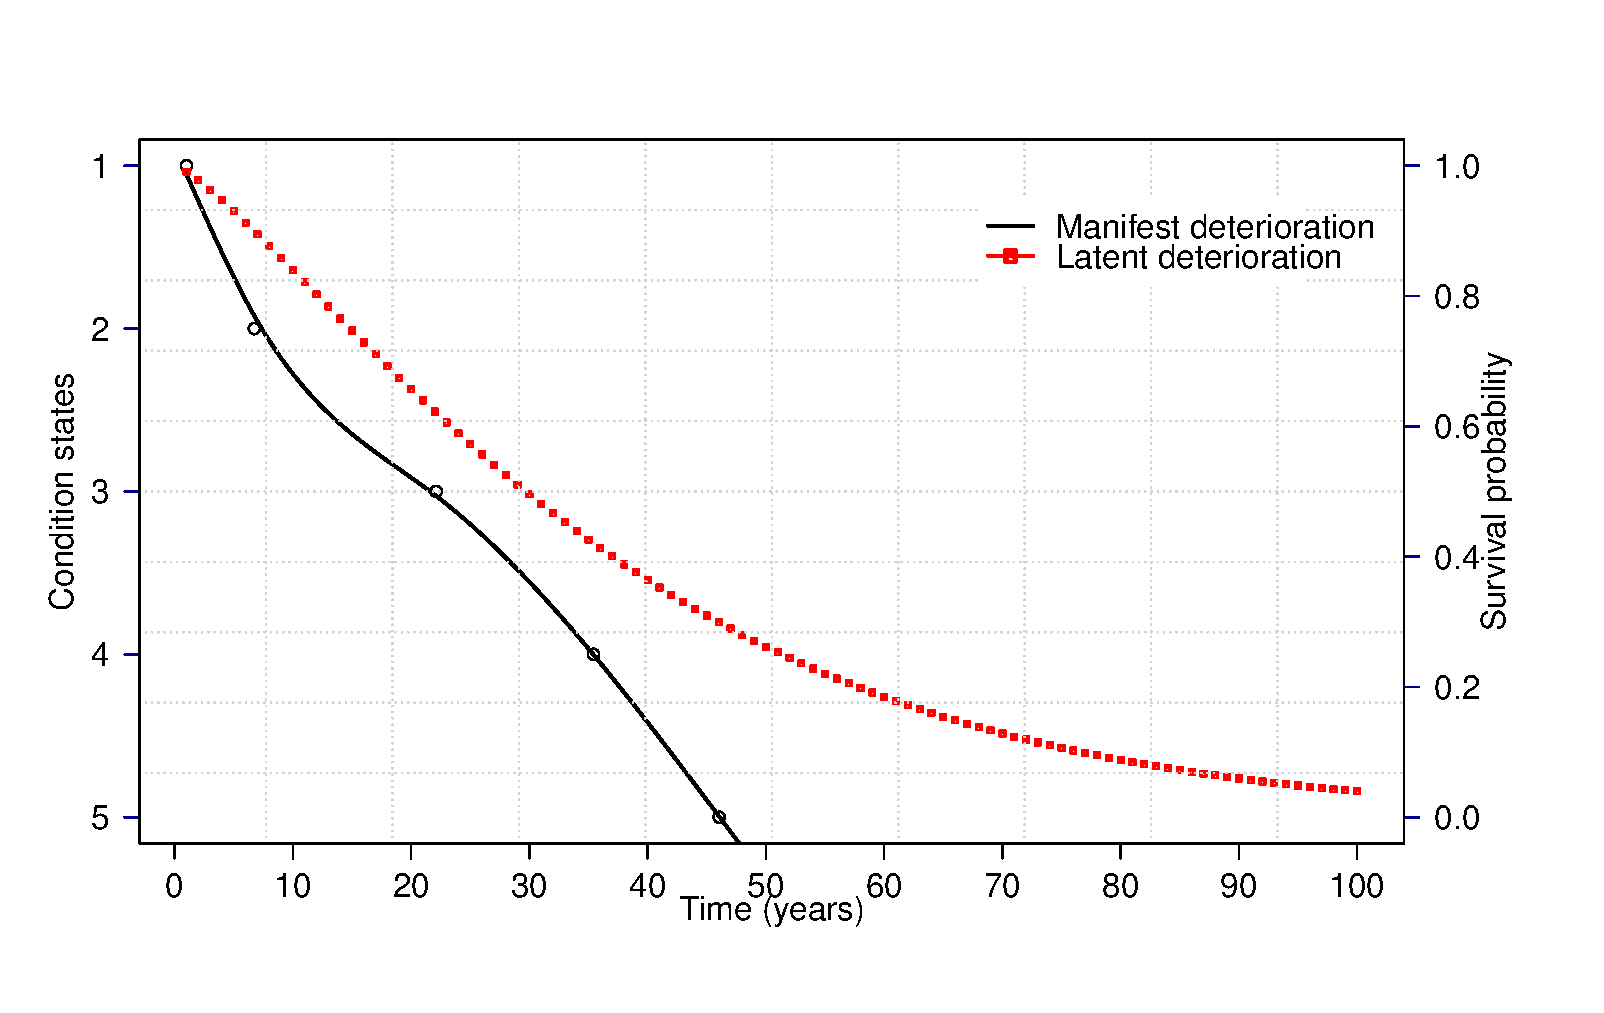
\includegraphics[scale=0.5]{fig1} 
\end{center} 
\caption{Deterioration process and visual inspection.} 
\label{fig1}
\end{figure} 

\section{Multi-state Markov Model}\label{section3}
In this section, we summary the research of \citeN{kobayashitsuda}, which proposes a modeling approach to estimate Markov transition probability based on visual inspection data. Careful readers are recommended to refer to the original paper for greater details of the methodology.

It is assumed that the deterioration status of a certain structure is provided as visual inspection data and its history performance path can be shown as in Fig. \ref{fig1}. In the figure, time $\tau$ represents the actual time on a calendar (hereafter refered as ''time''). Deterioration of an structure can be represented by discrete condition state $i(i=1,..,J)$, with $i=1$ as initial condition state (when structure is new) and $i=J$ as absorbing condition state. Time $\tau_A$ and $\tau_B$ are actual inspection times, while time $\tau_i$ is any arbitrary time in between. Duration between two inspection times is $Z$. Given monitoring data of two visual inspection times $\tau_A$ and $\tau_B$, the Markov transition probability can be described as follows:
\begin{eqnarray}
      && \hspace{-5mm}
      \mbox{Prob}[h(\tau_B)=j \hspace{2mm}| \hspace{2mm} h(\tau_A)=i]=p_{ij}
      \label{eq:1}
\end{eqnarray}
 %
Suppose that the deterioration status changes from $i$ to $i+1$ at time $\tau_{i}$ (timing $y_C$). At that time, the duration of the deterioration status $i$ can be expressed by the following equation: $\zeta_i=\tau_{i}-\tau_{i-1}=y_C$. Assume that the duration $\zeta_i$ of condition state $i$ is a random variable, and is subjected to the probability density function $f_i(\zeta_i)$ and the distribution function $F_i(\zeta_i)$. Here, the domain of the duration $\zeta_i$ is $[0,\infty)$. The following expression can be obtained from the definition of distribution function:
%
 \begin{eqnarray}
      && F_i(y_i)=\int_0^{y_i}f_i(\zeta_i)d\zeta_i
      \label{eq010}
   \end{eqnarray}
 %
The distribution function $F_i(y_i)$ represents the cumulative probability of the change of the condition state from $i$ to $i+1$ in the period from the initial timing $y_i=0$ (time $\tau_{i-1}$), at which the deterioration status has become $i$, to the timing $y_i$ (time $\tau_{i-1}+y_i$). Accordingly, the probability $\tilde{F}_i(y_i)$ of remaining at condition state $i$ from the initial timing $y_i=0$ to the sample timing $y_i\in [0,\infty)$ can be expressed by the following equation, using the cumulative probability of the change of the condition state from $i$ to $i+1$ until timing $y_i$:
 %
   \begin{eqnarray}
      && \mbox{Prob}\{\zeta_i \geq y_i\}= \tilde{F}_i(y_i) = 1 -  F_i(y_i)
      \label{funcbF}
   \end{eqnarray}
 %
The conditional probability of the event that the structure remains in condition state $i$ until timing $y_i$ and change to condition state $i+1$ in the period $[y_i,y_i+\Delta y_i)$ can be defined as:
 %
   \begin{eqnarray}
      && \lambda_i(y_i) \Delta y_i =\frac{f_i(y_i)\Delta y_i}{\tilde{F}_i(y_i)}
      \label{riskbF}
   \end{eqnarray}
 %
The instantaneous rate $\lambda_i(y_i)$ of the change in the condition state of the target structure from $i$ to $i+1$ at timing $y_i$ is called a hazard function. By using a hazard function suited for the assumed deterioration process, it is possible to describe initial failure, accidental deterioration, and deterioration with time, etc.

Under the assumption that the Markov characteristics concerning the deterioration processes of civil infrastructures do not depend on the history of deterioration and the hazard function is constant $\theta_i>0$, in another words, the hazard function is independent of the timing $y_i$, following equation is defined:
 %
   \begin{eqnarray}
      && \lambda_i(y_i)=\theta_i
      \label{hazard}
   \end{eqnarray}
 %
Using the hazard function $\lambda_i(y_i)=\theta_i$, the probability of the even that condition state $i$ remains over a duration $y_i$ can be further described as:
 %
   \begin{eqnarray}
      && \tilde{F}_i(y_i) = \exp \left[ - \int_{0}^{y_i}\lambda_i(u)du  \right]
       = \exp (-\theta_i y_i) \label{prop-bFla}
   \end{eqnarray}
%
The survival probability function is identical to the transition probability $p_{ii}$ when the duration $y_i$ equals to interval $z$. By defining the subsequent conditional probability of condition state $j$ to $i$, with respect to $z$, a general mathematical formula for estimating Markov transition probability $p_{ij}$ can be defined:
   \begin{eqnarray}
      && p_{ij}(z)=\mbox{Prob}[h(\tau_B)=j|h(\tau_A)=i] 
   =\sum_{k=i}^{j}\prod_{m=i}^{k-1}\frac{\theta_m}{\theta_{m}-\theta_{k}}
      \prod_{m=k}^{j-1}\frac{\theta_m}{\theta_{m+1}-\theta_{k}}
      \exp(-\theta_{k} z) \label{pj}
   \end{eqnarray}
 %
where there are the following conditions:
 %
   \begin{eqnarray}
      && \left\{
      \begin{array}{ll}
      \prod_{m=i}^{k-1}\frac{\theta_m}{\theta_m-\theta_k}=1 & at \hspace{2mm}(k\leq i+1)\\
      \prod_{m=k}^{j-1}\frac{\theta_m}{\theta_{m+1}-\theta_k}=1 & at \hspace{2mm}(k\geq j)
      \end{array}\right. 
   \end{eqnarray}
In addition, with regard to transition probability from any condition state to absorbing condition state $p_{iJ}$, following equation is used:
 %
   \begin{eqnarray}
      && p_{iJ}(z)=1-\sum_{j=i}^{J-1}p_{ij}(z)~(i=1,\cdots,J-1) \label{1pj}
   \end{eqnarray}
 %
The function of hazard $\theta_i$ can be expressed by means of function of characteristic variables $\mbox{\boldmath$x$}^k$ and unknown parameters $\mbox{\boldmath$\beta$}_i=(\beta_{i,1},\cdots,\beta_{i,M})$ ($M$ is number of characteristic variables and $k(k=1,...,K)$ is index of visual inspection data). 
   %
   \begin{eqnarray}
      && \theta_i^k=f(\mbox{\boldmath$x$}^k:\mbox{\boldmath$\beta$}_i)
      \label{hazard1}
   \end{eqnarray}
 %
Under the assumption of hazard function in Eq. (\ref{hazard1}), the Markov transition probability can be expressed by $p_{ij}(\bar{z}^k,\bar{\mbox{\boldmath$x$}}^k:\mbox{\boldmath$\beta$})$ as function of actual measurement data $(\bar{z}^k,\bar{\mbox{\boldmath$x$}}^k)$ and model's parameters (sometimes called unknown parameters) $\mbox{\boldmath$\beta$}=(\mbox{\boldmath$\beta$}_1,\cdots,\mbox{\boldmath$\beta$}_{J-1})$. Assuming that the deterioration phenomena of $K$ civil infrastructures are independent of one another, the likelihood function representing the probability density of the simultaneous occurrence of the deterioration transition pattern of all inspection samples can be formulated as follows \cite{tobin,amemi}:
 %
   \begin{eqnarray}
      && \hspace{-3mm} {\cal L}(\mbox{\boldmath$\beta$}) =
      \prod_{i=1}^{J-1} \prod_{j=i}^J\prod_{k=1}^{K}
      \left\{p_{ij}(\bar{z}^k,\bar{\mbox{\boldmath$x$}}^k:
      \mbox{\boldmath$\beta$})\right\}^{\bar{\delta}_{ij}^k}
      \label{logbF}
   \end{eqnarray}
 %
where $\delta_{ij}^k$ is dummy variable, having its value of $1$ when $h(\tau_A^k)=i$ and $h(\tau_B^k)=j$ and $0$ otherwise. Employing the MLE approach for the log likelihood function of Eq. (\ref{logbF}), parameter value $\beta$ can be estimated. As a result, hazard rate $\theta_i$ and Markov transition probability $p_{ij}$ can be obtained.

The expected duration of condition state $i$ can be defined by means of survival function $\tilde{F}_i(y_i^k)$ \cite{lancaster90}:
 %
   \begin{eqnarray}
      && R_i^k= \int^{\infty}_{0}\tilde{F}_i(y_i^k)dy_i^k= \int^{\infty}_{0}\exp (-\theta_i^k y_i^k) dy_i^k
      =\frac{1}{\theta_i^k} \label{17}
   \end{eqnarray}
 %
 %
\section{Bayesian Estimation Method}\label{section4}
\subsection{\textit{Bayes's theorem}}\label{section41}
In the Bayesian estimation, the posterior distribution of parameters is estimated by using the likelihood function, which is defined with the prior distribution of parameters and the observed data. Here, the likelihood function is represented by ${\cal L}(\mbox{\boldmath$\beta$}|\mbox{\boldmath$\xi$})$. $\mbox{\boldmath$\beta$}$ and $\mbox{\boldmath$\xi$}$ denote the unknown parameter vector and the observed data, respectively. 
It is assumed that $\mbox{\boldmath$\beta$}$ is a random variable, and is subject to the prior probability density function $\pi($\mbox{\boldmath$\beta$}$)$. Under these conditions and according to Baye's law, when the observed data $\mbox{\boldmath$\xi$}$ is given, the posterior probability density function $\pi($\mbox{\boldmath$\beta$}$|\mbox{\boldmath$\xi$})$ of the unknown parameters $\mbox{\boldmath$\beta$}$ can be defined as:
 %
   \begin{eqnarray}
      && \pi(\mbox{\boldmath$\beta$}|\mbox{\boldmath$\xi$})=
      \frac{{\cal L}(\mbox{\boldmath$\beta$}|\mbox{\boldmath$\xi$})
      \pi(\mbox{\boldmath$\beta$})}
      {\int_{\Theta}{\cal L}(\mbox{\boldmath$\beta$}|\mbox{\boldmath$\xi$})
      \pi(\mbox{\boldmath$\beta$})d\mbox{\boldmath$\beta$}}
      \label{bayes1}
   \end{eqnarray}
 %
where $\Theta$ represents the parameter space. At this time, $\pi($\mbox{\boldmath$\beta$}$|\mbox{\boldmath$\xi$})$ can be expressed as follows:
 %
   \begin{eqnarray}
      && \pi(\mbox{\boldmath$\beta$}|\mbox{\boldmath$\xi$})
      \propto {\cal L}(\mbox{\boldmath$\beta$}|\mbox{\boldmath$\xi$})
      \pi(\mbox{\boldmath$\beta$})
      \label{bayes2}
   \end{eqnarray}
 %
The symbol $\propto$ denotes 'be proportional to'. The denominator of the right-hand side of Eq. (\ref{bayes1}):
 %
   \begin{eqnarray}
      && m(\mbox{\boldmath$\xi$})
      =\int_{\Theta}{\cal L}(\mbox{\boldmath$\beta$}|\mbox{\boldmath$\xi$})
      \pi(\mbox{\boldmath$\beta$})d\mbox{\boldmath$\beta$}
      \label{bayes3}
   \end{eqnarray}
 %
is called the normalization constant of $\pi(\mbox{\boldmath$\beta$}|\mbox{\boldmath$\xi$})$, or the prior predictive distribution. In general, the procedures of the Bayesian estimation are as follows: 1) the prior probability distribution function $\pi(\mbox{\boldmath$\beta$})$ is specified, based on the prior information on experience, etc.; 2) the likelihood function ${\cal L}(\mbox{\boldmath$\beta$}|\mbox{\boldmath$\xi$})$ is defined based on the newly obtained data $\mbox{\boldmath$\xi$}$; and 3) the prior probability density function is modified in accordance with the Bayes' theorem, and the posterior probability density function $\pi(\mbox{\boldmath$\beta$}|\mbox{\boldmath$\xi$})$ regarding the parameters $\mbox{\boldmath$\beta$}$ is obtained. These procedures are called 'Bayesian estimation rule' in this study. The Bayesian estimation differs from the MLE method in that the probability distribution of the unknown parameters $\mbox{\boldmath$\beta$}$ is obtained as a posterior distribution.
\subsection{\textit{Bayesian estimation rule}}\label{section42}
This section discusses the method for estimating the parameter vector $\mbox{\boldmath$\beta$}$ of the multi-state Markov model with the Bayesian estimation rule, using the visual inspection data between two timings. The newly obtained data is represented by $\bar{\mbox{\boldmath$\xi$}}=(\bar{\mbox{\boldmath$\xi$}}^1,\cdots,\bar{\mbox{\boldmath$\xi$}}^K)$. In the Bayesian estimation of the multi-state Markov model, it is assumed that the available information for the inspection sample $k$ is $\bar{\mbox{\boldmath$\xi$}}^k=(\bar{\delta}_{ij}^k,\bar{z}^k,\bar{\mbox{\boldmath$x$}}^k)$. With refer to Eq. (\ref{pj}), the likelihood function in Eq. (\ref{logbF}) can be defined as:
 %
   \begin{eqnarray}
      && \hspace{-5mm} {\cal L}(\mbox{\boldmath$\beta$}|
      \bar{\mbox{\boldmath$\xi$}})
      =\prod_{i=1}^{J-1} \prod_{j=i}^J
      \prod_{k=1}^{K}\Big\{\sum_{h=i}^{j}\prod_{l=i}^{h-1}\frac{\theta^k_l}
      {\theta^k_{l}-\theta^k_{h}}
      \prod_{l=h}^{j-1}
      \frac{\theta^k_l}{\theta^k_{l+1}-\theta^k_{h}}
      \exp(-\theta^k_{h} \bar{z}^k)\Big\}^{\bar{\delta}_{ij}^k} \label{yuudo2}
   \end{eqnarray}
 %
In general, it is impossible to find a conjugate prior probability density function \cite{Lancaster2004} so that the functional form of the prior probability density function is identical with that of the posterior probability density function \cite{ibrahim01bo}. Here, it is assumed that the prior probability density function of $\mbox{\boldmath$\beta$}_i$ follows the multidimensional normal distribution $\mbox{\boldmath$\beta$}_i \sim {\cal N}_M(\mbox{\boldmath$\mu$}_i,\mbox{\boldmath$\Sigma$}_i)$, which is used as a standard prior probability density function. The probability density function of the $M$-dimensional normal distribution ${\cal N}_M(\mbox{\boldmath$\mu$}_i,\mbox{\boldmath$\Sigma$}_i)$ can be given by the following equation:
 %
   \begin{eqnarray}
      && \hspace{-2mm}
      g(\mbox{\boldmath$\beta$}_i|
      \mbox{\boldmath$\mu$}_i,\mbox{\boldmath$\Sigma$}_i)
      = \frac{1}{(2\pi)^{\frac{M}{2}}\sqrt{|\mbox{\boldmath$\Sigma$}_i|}}
      \cdot \exp\Big\{-\frac{1}{2}(\mbox{\boldmath$\beta$}_i
      -\mbox{\boldmath$\mu$}_i)
      \mbox{\boldmath$\Sigma_i$}^{-1}
      (\mbox{\boldmath$\beta$}_i-\mbox{\boldmath$\mu$}_i)^\prime\Big\}
            \label{Kseiki}
   \end{eqnarray}
 %
 %
where $\mbox{\boldmath$\mu$}_i$ represents the prior expectation vector of ${\cal N}_M(\mbox{\boldmath$\mu$}_i,\mbox{\boldmath$\Sigma$}_i)$, and $\mbox{\boldmath$\Sigma$}_i$ is the prior variance-covariance matrix. The symbol $\prime$ denotes transposition. At this time, the posterior probability density function $\pi(\mbox{\boldmath$\beta$}|\bar{\mbox{\boldmath$\xi$}})$ becomes as follows, based on Eq. (\ref{bayes2}):
 %
   \begin{eqnarray}
      && \hspace{-15mm} \pi(\mbox{\boldmath$\beta$}|\bar{\mbox{\boldmath$\xi$}})
      \propto {\cal L}(\mbox{\boldmath$\beta$}|\bar{\mbox{\boldmath$\xi$}})
      \prod_{i=1}^{J-1}g(\mbox{\boldmath$\beta$}_i|
      \mbox{\boldmath$\mu$}_i,\mbox{\boldmath$\Sigma$}_i)
      \propto \prod_{i=1}^{J-1} \prod_{j=i}^J \prod_{k=1}^{K}
      \Big\{\prod_{l=i}^{j-1}\theta^k_l\sum_{h=i}^{j}
      \prod_{l=i}^{h-1}\frac{1}{\theta^k_{l}-\theta^k_{h}}
      \nonumber \\
      && \cdot \prod_{l=h}^{j-1}\frac{1}{\theta^k_{l+1}-\theta^k_{h}}
      \exp(-\theta^k_{h} \bar{z}^k)\Big\}^{\bar{\delta}_{ij}^k}
       \cdot \prod_{i=1}^{J-1}\exp\Big\{-\frac{1}{2}
      (\mbox{\boldmath$\beta$}_i-\mbox{\boldmath$\mu$}_i)
      \mbox{\boldmath$\Sigma_i$}^{-1}
      (\mbox{\boldmath$\beta$}_i-\mbox{\boldmath$\mu$}_i)^\prime\Big\}
      \label{post1}
   \end{eqnarray}
 %
However, it is impossible to define the following normalization constant analytically, so there is no choice but to obtain the multiple integration value through numerical calculation.
 %
   \begin{eqnarray}
      && m(\bar{\mbox{\boldmath$\xi$}})
      =\int_{\Phi}{\cal L}(\mbox{\boldmath$\beta$}|\bar{\mbox{\boldmath$\xi$}})
      \prod_{i=1}^{J-1}g(\mbox{\boldmath$\beta$}_i|
      \mbox{\boldmath$\mu$}_i,\mbox{\boldmath$\Sigma$}_i)
      d \mbox{\boldmath$\beta$}
   \end{eqnarray}
 %
Generally, it is impossible to obtain the posterior probability density function $\pi(\mbox{\boldmath$\beta$}|\bar{\mbox{\boldmath$\xi$}})$ of the parameter vector $\mbox{\boldmath$\beta$}$ if using the MLE method. The next section proposes a methodology for directly obtaining the statistical values regarding the posterior distribution of parameters, using the MCMC method.
\subsection{\textit{Gibbs sampling}}\label{section43}
This section concerns the Gibbs sampling, which is a representative MCMC method \cite{Gamerman2006}. The Gibbs sampling method is a method for obtaining samples from the posterior distribution by generating randomly the samples of the parameters $\mbox{\boldmath$\beta$}$ repeatedly, using the conditional posterior probability density function. Particularly, when it is difficult to directly obtain the posterior probability density function $\pi(\mbox{\boldmath$\beta$}|\mbox{\boldmath$\xi$})$.
In order to explain the algorithm of the Gibbs sampling method, the observed data and the unknown parameter vector are represented by $\bar{\mbox{\boldmath$\xi$}}$ and $\mbox{\boldmath$\beta$}$. In addition, the unknown parameter vector subtracting $\beta_{e,m}$ from $\mbox{\boldmath$\beta$}$ is denoted by $\mbox{\boldmath$\beta$}^{-(e,m)}$. At this time, based upon the Eq. (\ref{post1}), the conditional posterior probability density function $\pi(\beta_{e,m}|\mbox{\boldmath$\beta$}^{-(e,m)},\bar{\mbox{\boldmath$\xi$}})$ of $\beta_{e,m}$ when $\mbox{\boldmath$\beta$}^{-(e,m)}$ is known as follows:
%
   \begin{manyeqns}
      && \pi(\beta_{e,m}|\mbox{\boldmath$\beta$}^{-(e,m)},
      \bar{\mbox{\boldmath$\xi$}})
      \propto \prod_{i=1}^{e} \prod_{j=e}^J\prod_{k=1}^{K}
      \Big\{{\theta^k_e}^{\bar{\delta}_{ij}^k-\bar{\delta}_{ie}^k}
      \cdot \sum_{h=i}^{j}\prod_{l=i}^{h-1}\frac{1}{\theta^k_{l}-\theta^k_{h}}
      \prod_{l=h}^{j-1}\frac{1}{\theta^k_{l+1}-\theta^k_{h}}
      \exp(-\theta^k_{h} \bar{z}^k)\Big\}^{\bar{\delta}_{ij}^k} \nonumber \\
 %
      && \hspace{25mm}
      \cdot \exp\Big\{-\frac{1}{2}
      (\mbox{\boldmath$\beta$}_e-\mbox{\boldmath$\mu$}_e)
      \mbox{\boldmath$\Sigma_e$}^{-1}
      (\mbox{\boldmath$\beta$}_e-\mbox{\boldmath$\mu$}_e)^\prime \Big\} \\
      && \hspace{2mm} \propto \prod_{i=1}^{e} \prod_{j=e}^J\prod_{k=1}^{K}
      \Big\{{\exp{(\beta_{e,m}x^k_{m})}}^
      {\bar{\delta}_{ij}^k-\bar{\delta}_{ie}^k}
      \cdot \sum_{h=i}^{j}\prod_{l=i}^{h-1}\frac{1}{\theta^k_{l}-\theta^k_{h}}
      \prod_{l=h}^{j-1}\frac{1}{\theta^k_{l+1}-\theta^k_{h}}
      \exp(-\theta^k_{h} \bar{z}^k) \Big\}^{\bar{\delta}_{ij}^k}
      \nonumber \\
      && \hspace{25mm} \cdot
      \exp\Big\{-\frac{\rho_{e}^{mm}}{2}(\beta_{e,m}-\hat{\mu}_{e}^m)^2 \Big\}
      \label{condition1} \\
      && \hspace{20mm}
      \hat{\mu}_{e}^m
      = \mu_{e}^m+\sum_{h=1,\neq m}^{M}(\beta_{e,h}-\mu_{e}^h)\rho_e^{hm}
\end{manyeqns}
%
%
where $\bar{\delta}_{ie}^k$ is a dummy variable, which is 1 when the prior condition state $d(\tau_A^k)=i$ of the inspection sample $k$ is equal to the prior condition state of the Gibbs sampling $e$ and 0 when they are different. $\mu_{e}^m$ is the $m$-th element of the prior expectation vector $\mbox{\boldmath$\mu$}_e$, and $\rho_{e}^{hm}$ is the $(h,m)$-th element of the prior variance-covariance matrix $\mbox{\boldmath$\Sigma_e$}^{-1}$. In addition, $\sum_{h=1,\neq m}^{M}$ means the sum of the elements from 1 to $M$, excluding $m$. It is possible to generate samples from these conditional probability density functions, and calculate statistical values regarding the posterior distribution of the parameters $\mbox{\boldmath$\beta$}$ using the samples. In short, the Gibbs sampling algorithm can be summarized in following steps:
\begin{description}
\item       step1: Specify the initial parameter {\small $\mbox{\boldmath$\beta$}{(0)}=(\beta_{1,1}{(0)},\cdots,\beta_{J-1,M}{(0)})$}. Set $n=1$, and the number of samples $\overline{n}$.
\item       step2: Generate  $\mbox{\boldmath$\beta$}{(n)}=(\beta_{1,1}{(n)},\cdots,\beta_{J-1,M}{(n)})$ as follows:\\
      Generate $\beta_{1,1}$ randomly from $\pi(\beta_{1,1}|\mbox{\boldmath$\beta$}^{-(1,1)}{(n-1)},
      \bar{\mbox{\boldmath$\xi$}})$.\\
      Generate $\beta_{1,2}$ randomly from $\pi(\beta_{1,2}|\mbox{\boldmath$\beta$}^{-(1,2)}{(n-1)},\bar{\mbox{\boldmath$\xi$}})$.\\
      ----- \\
      Generate $\beta_{e,m}$ randomly from $\pi(\beta_{e,m}|\mbox{\boldmath$\beta$}^{-(e,m)}{(n-1)},\bar{\mbox{\boldmath$\xi$}})$.\\
      ----- \\
      Generate $\beta_{J-1,M}$ randomly from $\pi(\beta_{J-1,M}|\mbox{\boldmath$\beta$}^{-(J-1,M)}{(n-1)},\bar{\mbox{\boldmath$\xi$}})$
\item step 3: When $\underline{n}$ is sufficiently large and $n>\underline{n}$, record $\mbox{\boldmath$\beta$}{(n)}$.
\item step 4: When $n=N$, terminate the calculation. If $n<\overline{n}$, set $n=n+1$, and return to Step 2.
\end{description}
In the above Gibbs sampling, the transition kernel is defined as follows:
 %
   \begin{eqnarray}
      && \hspace{-5mm}
      K(\mbox{\boldmath$\beta$}{(n-1)},\mbox{\boldmath$\beta$}{(n)}|
      \bar{\mbox{\boldmath$\xi$}}) 
       =\prod_{e=1}^{J-1}\prod_{m=1}^{M}
      \pi(\beta_{e,m}(n)|\mbox{\boldmath$\beta$}^{-(e,m)}
      {(n-1)},\bar{\mbox{\boldmath$\xi$}}) \label{suii}
   \end{eqnarray}
 %
 %
Where $\mbox{\boldmath$\beta$}{(n)} ~(n=0,1,\cdots)$ is the Markov chain containing the transition kernel $K(\mbox{\boldmath$\beta$}{(n-1)}$, $\mbox{\boldmath$\beta$}{(n)}|\bar{\mbox{\boldmath$\xi$}})$. In addition, the steady state of this Markov chain is represented by $\pi(\mbox{\boldmath$\beta$}|\bar{\mbox{\boldmath$\xi$}})$. Assuming that the Markov chain has reached the steady state while $\underline{n}$ is sufficiently large, it is possible to consider $\mbox{\boldmath$\beta$}(n)~(n=\underline{n}+1,\underline{n}+2,\cdots,\overline{n})$, which has been obtained in the Gibbs sampling, as the sample from the posterior probability density function $\pi(\mbox{\boldmath$\beta$}|\bar{\mbox{\boldmath$\xi$}})$. Accordingly, by using these samples, it is possible to calculate the statistical values regarding the posterior distribution of the parameter vector $\mbox{\boldmath$\beta$}$. In order to conduct the Gibbs sampling, it is necessary to obtain $(J-1)�~M$ conditional posterior probability density functions $\pi(\beta_{e,m}|\mbox{\boldmath$\beta$}^{-(e,m)},\bar{\mbox{\boldmath$\xi$}})~(e=1,\cdots,J-1,m=1,\cdots,M)$. In general, adaptive rejection sampling (ARS) \cite{gilks} is effective as a method for obtaining samples from a probability density function $f(x)$, whose $\ln [f(x)]$ becomes a concave function. It is possible to verify that the conditional posterior probability density function $\pi(\beta_{e,m}|\mbox{\boldmath$\beta$}^{-(e,m)},\bar{\mbox{\boldmath$\xi$}})$ does not satisfy the above mentioned characteristics, but in many cases, $\ln [\pi(\beta_{e,m}|\mbox{\boldmath$\beta$}^{-(e,m)},\bar{\mbox{\boldmath$\xi$}})]$ is regarded as a logarithmic concave function, and so this study adopts the ARS as a method for sampling the parameters $\mbox{\boldmath$\beta$}$ of the posterior distribution from Eq. (\ref{condition1}).

\subsection{\textit{Setting of a priori distribution}}\label{section44}
When conducting the Bayesian estimation of the multi-state Markov model, the prior information possessed by engineers can be expressed as a prior distribution. However, as mentioned above, there is no conjugate prior distribution in which the functional form of the prior distribution becomes the same as that of the posterior distribution. Therefore, it can be considered that the prior distribution based on prior experience does not represent the true probability density of unknown parameters. However, it is referred to as a tool for representing the past estimation results and the technical information possessed by engineers. In this study, the prior probability density function of the unknown parameters $\mbox{\boldmath$\beta$}_i~(i=1,\cdots,J-1)$ of the multi-state Markov  model is assumed to follow multidimensional normal distribution  $\mbox{\boldmath$\beta$}_i \sim {\cal N}_M(\mbox{\boldmath$\mu$}_i,\mbox{\boldmath$\Sigma$}_i)$. By assuming such a relatively simple prior probability density function, it is possible to express the prior knowledge as the prior distribution in a simple form.

On the other hand in the case of no information on the expectation or variance of the parameter vector $\mbox{\boldmath$\beta$}$, it is possible to use the following prior distribution whose variance is sufficiently large \cite{ibrahim01bo}:
 %
   \begin{eqnarray}
      && \mbox{\boldmath$\beta$}_i \sim {\cal N}_M
      (\mbox{\boldmath$O$},\kappa_{\beta_{i}} \mbox{\boldmath$I$})
      \label{nn2}
   \end{eqnarray}
 %
where $\kappa_{\beta_i}$ is a sufficiently large positive number. In addition, $\mbox{\boldmath$O$}$ and $\mbox{\boldmath$I$}$ represent the zero vector, whose elements are all zero, and the unit matrix, respectively. It is also possible to use the following Jeffreys-type non-informative prior distribution \cite{Jeffreys1961}: %
   \begin{eqnarray}
      && g(\beta_{i,m}) \propto \tilde{\beta}_{i,m}
      \label{sei2}
   \end{eqnarray}
 %
where $\tilde{\beta}_{i,m}$ is an arbitrary constant that satisfies the condition: $-\infty< \tilde{\beta}_{i,m} <\infty$. Here, the Jeffreys-type non-informative prior distribution is called a non-holomorphic prior distribution, because it does not become 1 even when integrated in the domain of definition. A non-holomorphic prior distribution is not a probability density function, but it is possible to obtain a posterior distribution based on the Bayesian estimation rule, using a non-holomorphic priori distribution in Eq. (\ref{sei2}) \cite{Gamerman2006,Jeffreys1961}. That is, using the Jeffreys-type non-informative prior distribution, the conditional posterior probability density function in Gibbs sampling can be expressed as:
 %
   \begin{eqnarray}
      && \pi(\beta_{e,m}|\mbox{\boldmath$\beta$}^{-(e,m)},
      \bar{\mbox{\boldmath$\xi$}}) \nonumber \\
      && \hspace{0mm} \propto \prod_{i=1}^{e} \prod_{j=e}^J\prod_{k=1}^{K}
      \Big\{{\exp{(\beta_{e,m}x^k_{m})}}
      ^{\bar{\delta}_{ij}^k-\bar{\delta}_{ie}^k}
        \cdot \sum_{h=i}^{j}\prod_{l=i}^{h-1}\frac{1}{\theta^k_{l}-\theta^k_{h}}
      \prod_{l=h}^{j-1}\frac{1}{\theta^k_{l+1}-\theta^k_{h}}
      \exp(-\theta^k_{h} \bar{z}^k) \Big\}^{\bar{\delta}_{ij}^k}
          \label{condi2}
   \end{eqnarray}
 %
Eq. (\ref{condi2}) shows the proportional relation, and so the Jeffreys-type non-informative parameter has been deleted from the right-hand side. As mentioned here, the conditional posterior probability density function used in Gibbs sampling varies according to the type of available prior information.
\subsection{\textit{Statistics values regarding the posterior distribution}}
Based on the samples obtained through the MCMC method, it is possible to analyze the statistical characteristics of the parameter vector $\mbox{\boldmath$\beta$}$. Moreover, with the MCMC method, it is also possible to express the posterior probability density function $\pi(\mbox{\boldmath$\beta$}|\mbox{\boldmath$\xi$})$ as an analytical function. Using the obtained samples, the distribution function and the density function are estimated in a non-parametric manner. Here, the samples obtained through the Gibbs sampling are represented by $\mbox{\boldmath$\beta$}(n)~(n=1,\cdots,\overline{n})$, where $\mbox{\boldmath$\beta$}(n)=(\mbox{\boldmath$\beta$}_1(n),\cdots,\mbox{\boldmath$\beta$}_{J-1}(n))$. Among them, the first $\underline{n}$ samples are considered as the samples from the convergent process, and removed from the sample set. Then, the sample suffix set of parameters is defined as ${\cal M}=\{\underline{n}+1,\cdots,\overline{n})$. At this time, the joint probability density function $G(\mbox{\boldmath$\beta$})$ of the parameters $\mbox{\boldmath$\beta$}$ can be expressed by the following equation:
 %
   \begin{eqnarray}
      && G(\mbox{\boldmath$\beta$})
      =\frac{\mbox{\#}(\mbox{\boldmath$\beta$}(n)
      \leq \mbox{\boldmath$\beta$}, n\in {\cal M})}
      {\overline{n}-\underline{n}}
   \end{eqnarray}
 %
where $\mbox{\#}(\mbox{\boldmath$\beta$}(n) \leq \mbox{\boldmath$\beta$}, n\in {\cal M})$ represents the sum of samples satisfying the logical formula: $\mbox{\boldmath$\beta$}(n) \leq \mbox{\boldmath$\beta$}, n\in {\cal M}$. In addition, the expectation vector $\tilde{\mbox{\boldmath$\mu$}_i}(\mbox{\boldmath$\beta$}_i)$ and the variance-covariance matrix $\tilde{\mbox{\boldmath$\Sigma$}_i}(\mbox{\boldmath$\beta$}_i)$ of the posterior distribution of the parameters $\mbox{\boldmath$\beta$}_i$ can be expressed by the following equations:
 %
   \begin{manyeqns}
      && \hspace{-7mm}
      \tilde{\mbox{\boldmath$\mu$}_i}(\mbox{\boldmath$\beta$}_i)=
      (\tilde{\mu}(\beta_{i,1}),\cdots,\tilde{\mu}
      (\beta_{i,M}))^\prime 
       =\Big(\sum_{n=\underline{n}+1}^{\overline{n}}
      \frac{\beta_{i,1}(n)}{\overline{n}-\underline{n}},
      \cdots, \sum_{n=\underline{n}+1}^{\overline{n}}
      \frac{\beta_{i,M}(n)}{\overline{n}-\underline{n}}\Big)^\prime
      \label{mu3} \\
 %
      && \hspace{-7mm}
      \tilde{\mbox{\boldmath$\Sigma$}_i}(\mbox{\boldmath$\beta$}_i)=
      \left(
      \begin{array}{lll}
         \tilde{\sigma}^2(\beta_{i,1}) & \cdots
            & \tilde{\sigma}(\beta_{i,1}\beta_{i,M}) \\
         \vdots & \ddots & \vdots \\
         \tilde{\sigma}(\beta_{i,M}\beta_{i,1}) & \cdots
            & \tilde{\sigma}^2(\beta_{i,M}) \\
      \end{array}
      \right)
      \label{mu4}
   \end{manyeqns}
 %
where
 %
   \begin{manyeqns}
      && \hspace{-3mm} \tilde{\sigma}^2(\beta_{i,m})=
      \sum_{n=\underline{n}+1}^{\overline{n}}
      \frac{\{\beta_{i,m}(n)-\tilde{\mu}(\beta_{i,m})\}^2}
      {\overline{n}-\underline{n}} \\
      && \hspace{-3mm} \tilde{\sigma}(\beta_{i,m}\beta_{i,l}) 
      =\sum_{n=\underline{n}+1}^{\overline{n}}
      \frac{\{\beta_{i,m}(n)-\tilde{\mu}(\beta_{i,m})\}
      \{\beta_{i,l}(n)-\tilde{\mu}(\beta_{i,l})\}}{\overline{n}-\underline{n}}
            \end{manyeqns}
 %
The $100(1-2\alpha)\%$ confidence interval can be defined as $\underline{\beta}^{\alpha}_{i,m}< \beta_{i,m} <\overline{\beta}^{\alpha}_{i,m}$, using the sample order statistic $(\underline{\beta}^{\alpha}_{i,m},\overline{\beta}^{\alpha}_{i,m})~(i=1,\cdots,J-1, \quad m=1,\cdots,M)$:
 %
   \begin{manyeqns}
      && \hspace{-8mm} \underline{\beta}^{\alpha}_{i,m}
      =\arg \max_{\beta_{i,m}(n^\ast)} 
       \left\{ \frac{\#(\beta_{i,m}(n) \leq \beta_{i,m}(n^\ast),n
      \in {\cal M})}
      {\overline{n}-\underline{n}}\leq \alpha \right\} \\
 %
      && \hspace{-8mm} \overline{\beta}^{\alpha}_{i,m}
      =\arg \min_{\beta_{i,m}(n^{\ast\ast})} 
       \left\{ \frac{\#(\beta_{i,m}(n) \geq
      \beta_{i,m}(n^{\ast\ast}),n\in {\cal M})}
      {\overline{n}-\underline{n}}\leq \alpha \right\}
   \end{manyeqns}
\subsection{\textit{Bayesian updating rule}}\label{section45}
In the Bayesian estimation, if there exists a conjugate prior distribution while the prior and posterior distributions have the same functional form, it is possible to update the Bayesian estimates of unknown parameters, using the newly obtained data. However, in the case of the multi-state Markov model, the conjugate prior distribution does not exist. Therefore, when the Bayesian updating is conducted, it is necessary to accumulate all past inspection data that are used for the model estimation.

Here, consider a case in which the posterior distribution in Eq. (\ref{post1}) regarding the unknown parameters of the multi-state Markov model has been obtained, using the first inspection data $\bar{\mbox{\boldmath$\xi$}}^0$. Then, discuss the problem of updating the posterior distribution of the unknown parameters, using the second inspection data $\bar{\mbox{\boldmath$\xi$}}^1$. The available information regarding the inspection sample $k$ is $\mbox{\boldmath$\xi$}^k=(\bar{\delta}_{ij}^k,\bar{z}^k,\bar{\mbox{\boldmath$x$}}^k)$. In addition, the database pooling the first inspection data $\bar{\mbox{\boldmath$\xi$}}^0=(\bar{\delta}_{ij}^k,\bar{z}^k,\bar{\mbox{\boldmath$x$}}^k)~(k=1,\cdots,k_1)$ and the second inspection data $\bar{\mbox{\boldmath$\xi$}}^1=(\bar{\delta}_{ij}^k,\bar{z}^k,\bar{\mbox{\boldmath$x$}}^k)~(k=k_1+1,\cdots,k_1+k_2)$ is defined. Assuming that the posterior probability density function of the unknown parameter vector in the first Bayesian estimation is $\pi(\mbox{\boldmath$\beta$}|\bar{\mbox{\boldmath$\xi$}}^0)$, the posterior density function $\pi(\mbox{\boldmath$\beta$}|\bar{\mbox{\boldmath$\xi$}}^0,\bar{\mbox{\boldmath$\xi$}}^1)$ of the unknown parameter vector after the Bayesian updating can be expressed as follows:
 %
   \begin{eqnarray}
      \pi(\mbox{\boldmath$\beta$}|\bar{\mbox{\boldmath$\xi$}}^0,
      \bar{\mbox{\boldmath$\xi$}}^1)
      &&\propto {\cal L}(\mbox{\boldmath$\beta$}|\bar{\mbox{\boldmath$\xi$}}^1)
      \pi(\mbox{\boldmath$\beta$}|\bar{\mbox{\boldmath$\xi$}}^0) 
      \propto {\cal L}(\mbox{\boldmath$\beta$}|\bar{\mbox{\boldmath$\xi$}}^0,
      \bar{\mbox{\boldmath$\xi$}}^1)
      \prod_{i=1}^{J-1}g(\mbox{\boldmath$\beta$}_i|\mbox{\boldmath$\mu$}_i,
      \mbox{\boldmath$\Sigma$}_i)
   \end{eqnarray}
 %
 %
where ${\cal L}(\mbox{\boldmath$\beta$}|\bar{\mbox{\boldmath$\xi$}}^0,\bar{\mbox{\boldmath$\xi$}}^1)$ is the likelihood function defined by using the database pooling the data of the first and second inspections. On the other hand, $g(\mbox{\boldmath$\beta$}_i|\mbox{\boldmath$\mu$}_i,\mbox{\boldmath$\Sigma$}_i)$ represents the prior distribution of $\mbox{\boldmath$\beta$}_i$ used in the first Bayesian estimation. Accordingly, the posterior distribution after the Bayesian updating becomes as follows:
 %
   \begin{eqnarray}
      && \hspace{0mm} \pi(\mbox{\boldmath$\beta$}|
      \bar{\mbox{\boldmath$\xi$}}^0,\bar{\mbox{\boldmath$\xi$}}^1)
      \propto \prod_{i=1}^{J-1} \prod_{j=i}^J\prod_{k=1}^{k_1+k_2}
      \Big\{\prod_{l=i}^{j-1}\theta^k_l 
       \cdot \sum_{h=i}^{j}\prod_{l=i}^{h-1}
      \frac{1}{\theta^k_{l}-\theta^k_{h}}
      \prod_{l=h}^{j-1}\frac{1}{\theta^k_{l+1}-\theta^k_{h}}
      \exp(-\theta^k_{h} \bar{z}^k)\Big\}^{\bar{\delta}_{ij}^k} \nonumber \\
      && \cdot \prod_{i=1}^{J-1}\exp\Big\{-\frac{1}{2}
      (\mbox{\boldmath$\beta$}_i-\mbox{\boldmath$\mu$}_i)
      \mbox{\boldmath$\Sigma_i$}^{-1}
      (\mbox{\boldmath$\beta$}_i-\mbox{\boldmath$\mu$}_i)^\prime\Big\}
      \label{postu2}
   \end{eqnarray}
 %
 %
That is, as obvious from Eq. (\ref{postu2}), in order to update the posterior distribution of the unknown parameters, it is necessary to define a likelihood function for the database with new inspection data, and obtain a posterior distribution by Gibbs sampling. Also when a non-informative prior distribution is used, it is possible to update the posterior distribution of the unknown parameters through Gibbs sampling, by defining a likelihood function for the database with new additional data.

\section{Empirical Study}\label{section5}
\subsection{\textit{Outline}}\label{section51}
In order to discuss the effectiveness of the methodology proposed in this study, the Bayesian estimation of the multi-state Markov model is attempted, using the visual inspection data of bridges managed by N city. This section briefly describes the visual inspection and inspection data of the bridges in N city. As a concrete target for the Bayesian estimation, this section focuses on RC slabs, on which loading is directly imposed and which are important members. Table \ref{table1} shows the evaluation criteria for the $7$ condition states in the visual inspection of RC slabs. The amount of accumulated data in N city is enormous, and the number of inspection data obtained from the two successive timings amounts to 32,902. However, in reality, the database does not have such a plentiful amount of inspection samples in many cases. Then, the second database is produced by extracting samples from such database, and the effectiveness of the proposed Bayesian estimation is empirically examined.

  \begin{table}[t]
   \begin{center}
      \caption{Evaluation Criteria for $7$ condition states}
      \label{table1}
      {\small
      \begin{tabular}{c|l}\hline
      
      & \multicolumn{1}{|c}{Physical meaning(RC slab)} \\ \hline

      1 & Newly established state. There is no sign\\
        & of deterioration.\\
      2 & Intermediate level between '1' and '3'\\
      3 & Water leakage is observed at part of the\\
        & slab. (Unidirectional cracking accompanied\\
        & by water leakage, and spotted water\\
        & leakage at the edges)\\
      4 & Intermediate level between '3' and '5'\\
      5 & Water leakage is observed in over 75$\%$ of\\
        & the slab area. Peeling and falling are\\
        & observed at part of the slab. Free lime is\\
        & observed along the flange on the girder.\\
      6 & Intermediate level between '5' and '7' \\
      7 & Serious peeling and free lime are observed.\\
        & Slab part falling or its sign is observed.\\\hline
      \end{tabular}
      }
      \end{center}

\end{table}
 %

\subsection{\textit{Effectiveness of the Gibbs sampling}}\label{section52}
The exponential hazard function used for the Bayesian estimation is specified as follows:
 %
   \begin{eqnarray}
      && \theta_i^k=\exp{(\beta_{i,1}+ \beta_{i,2}x_2^k +\beta_{i,3}x_3^k)}
      \label{bgutai} \\
      && (i=1,\cdots,6; k=1,\cdots,K) \nonumber
   \end{eqnarray}
 %
For the explanatory variables in the above Eq. (\ref{bgutai}), the explanatory variable pair selected in the reference \cite{kobayashitsuda} is adopted without any modification. For $x_2^k$ and $x_3^k$, the average traffic volume and the slab area of the RC slab $k$ are adopted. The expression $\mbox{\boldmath$\beta$}_i=(\beta_{i,1},\beta_{i,2},\beta_{i,3})$ is used. In Eq. (\ref{bgutai}), in order to automatically satisfy the constraint condition $\theta_i^k > 0$, the exponential function-based regression equation is employed.

\begin{table}[t]
\begin{center}
\caption{Result of the Bayesian estimation (using the original database).}
\label{table2}
{\footnotesize
\begin{tabular}{l|lll|lll}
\hline
\multicolumn{1}{c|}{Condition} & \multicolumn{3}{c|}{Prior distribution of Eq. (\ref{initial2})} & \multicolumn{3}{c}{Non-information prior distribution} \\ 
\cline{2-7}
\multicolumn{1}{c|}{states} & \multicolumn{1}{c}{Constant term} & \multicolumn{1}{c}{TV} & \multicolumn{1}{c|}{Slab area} & \multicolumn{1}{c}{Constant term} & \multicolumn{1}{c}{TV} & \multicolumn{1}{c}{Slab area} \\ 
\multicolumn{1}{c|}{} & \multicolumn{1}{c}{$\beta_{i,1}$} & \multicolumn{1}{c}{$\beta_{i,2}$} & \multicolumn{1}{c|}{$\beta_{i,3}$} & \multicolumn{1}{c}{$\beta_{i,1}$} & \multicolumn{1}{c}{$\beta_{i,2}$} & \multicolumn{1}{c}{$\beta_{i,3}$} \\ 
\hline
\multicolumn{1}{c|}{1} & \multicolumn{1}{c}{-1.078} & \multicolumn{1}{c}{-} & \multicolumn{1}{c|}{1.389} & \multicolumn{1}{c}{-1.100} & \multicolumn{1}{c}{-} & \multicolumn{1}{c}{2.854} \\ 
\multicolumn{1}{c|}{} & \multicolumn{1}{c}{(1.010)} & \multicolumn{1}{c}{-} & \multicolumn{1}{c|}{(0.110)} & \multicolumn{1}{c}{(0.160)} & \multicolumn{1}{c}{-} & \multicolumn{1}{c}{(0.160)} \\ 
\hline
\multicolumn{1}{c|}{2} & \multicolumn{1}{c}{-1.549} & \multicolumn{1}{c}{0.255} & \multicolumn{1}{c|}{2.662} & \multicolumn{1}{c}{-1.555} & \multicolumn{1}{c}{0.237} & \multicolumn{1}{c}{3.033} \\ 
\multicolumn{1}{c|}{} & \multicolumn{1}{c}{(0.990)} & \multicolumn{1}{c}{(0.920)} & \multicolumn{1}{c|}{(0.040)} & \multicolumn{1}{c}{(0.800)} & \multicolumn{1}{c}{(0.910)} & \multicolumn{1}{c}{(1.050)} \\ 
\hline
\multicolumn{1}{c|}{3} & \multicolumn{1}{c}{-1.970} & \multicolumn{1}{c}{0.690} & \multicolumn{1}{c|}{-} & \multicolumn{1}{c}{-1.973} & \multicolumn{1}{c}{0.699} & \multicolumn{1}{c}{-} \\ 
\multicolumn{1}{c|}{} & \multicolumn{1}{c}{(1.200)} & \multicolumn{1}{c}{(1.160)} & \multicolumn{1}{c|}{-} & \multicolumn{1}{c}{(0.270)} & \multicolumn{1}{c}{(1.240)} & \multicolumn{1}{c}{-} \\ 
\hline
\multicolumn{1}{c|}{4} & \multicolumn{1}{c}{-2.432} & \multicolumn{1}{c}{0.824} & \multicolumn{1}{c|}{0.498} & \multicolumn{1}{c}{-2.422} & \multicolumn{1}{c}{0.849} & \multicolumn{1}{c}{0.506} \\ 
\multicolumn{1}{c|}{} & \multicolumn{1}{c}{(1.530)} & \multicolumn{1}{c}{(1.470)} & \multicolumn{1}{c|}{(0.230)} & \multicolumn{1}{c}{(0.970)} & \multicolumn{1}{c}{(1.100)} & \multicolumn{1}{c}{(0.980)} \\ 
\hline
\multicolumn{1}{c|}{5} & \multicolumn{1}{c}{-2.316} & \multicolumn{1}{c}{-} & \multicolumn{1}{c|}{-} & \multicolumn{1}{c}{-2.322} & \multicolumn{1}{c}{-} & \multicolumn{1}{c}{-} \\ 
\multicolumn{1}{c|}{} & \multicolumn{1}{c}{(0.940)} & \multicolumn{1}{c}{-} & \multicolumn{1}{c|}{-} & \multicolumn{1}{c}{(0.210)} & \multicolumn{1}{c}{-} & \multicolumn{1}{c}{-} \\ 
\hline
\multicolumn{1}{c|}{6} & \multicolumn{1}{c}{-1.882} & \multicolumn{1}{c}{1.279} & \multicolumn{1}{c|}{-} & \multicolumn{1}{c}{-1.955} & \multicolumn{1}{c}{1.538} & \multicolumn{1}{c}{-} \\ 
\multicolumn{1}{c|}{} & \multicolumn{1}{c}{(0.510)} & \multicolumn{1}{c}{(0.900} & \multicolumn{1}{c|}{-} & \multicolumn{1}{c}{(0.030)} & \multicolumn{1}{c}{(0.090)} & \multicolumn{1}{c}{-} \\ 
\hline
\multicolumn{1}{c|}{Log-likelihood} & \multicolumn{3}{c|}{-20062} & \multicolumn{3}{c}{-20060} \\ 
\hline
\end{tabular}
}
\end{center}
\footnotesize Note) TV stands for average traffic volume
\end{table}

Table \ref{table2} shows the results of the Bayesian estimation of the multi-state Markov model (sample average of parameters), using the prior distribution setting the prior information as
 %
   \begin{eqnarray}
      &&\mbox{\boldmath$\beta$}_i \sim {\cal N}_3
      (\mbox{\boldmath$O$},\mbox{\boldmath$I$})
       \label{initial2}
   \end{eqnarray}
 %
In addition, the $\cal Z$-score in Geweke test statistic \cite{geweke} is also shown. For conducting Gibbs sampling, the number of samples for the Markov chain to reach the steady state is set as $\underline{n}=3,000$. As shown in Table \ref{table2}, the Geweke test statistic ${\cal Z}_{\beta_{i,m}}$ is less than 1.96, so it is obvious that the convergent hypothesis cannot be nullified with the 5\% significance level. In the following calculations, suppose $\overline{n}=13,000$, $\underline{n}=3,000$ samples are removed as the samples from the process of converging to the posterior distribution, and the analysis is carried out by using the remaining 10,000 parameter samples. 

For comparison, Table \ref{table4} also shows the estimation results of the model by applying the MLE method, using the original database. A greater detail of using the MLE method is explained in the paper of \citeN{kobayashitsuda}. In the case where the probability density function of the prior distribution regarding all parameters is positive and gentle in the domain, the posterior distribution approaches asymptotically to a normal distribution whose mean is the MLE estimate and variance is the inverse of Fisher Information. 

As shown in Table \ref{table2}, when the original database and the prior distribution of Eq. (\ref{initial2}) are used, the sample mean is nearly equal to the maximum-likelihood estimate shown in Table \ref{table3} for most parameters, and it is obvious that the Gibbs sampling is conducted efficiently. However, there exist parameters whose sample mean and maximum-likelihood estimate are different from each other. This is considered due to the fact that the Gibbs sampling data is not enough to make the maximum-likelihood estimate equal to the mean of the posterior distribution. One of the reasons why Gibbs sampling is inefficient is that the variance of the prior distribution is small. Here, as shown in Table \ref{table2} and Table \ref{table3}, there is little difference in log likelihood among the models. 

Table \ref{table2} also shows the results of the Bayesian estimation with the non-informative prior distribution (\ref{sei2}). The non-informative prior distribution can be obtained by setting the variance of the prior distribution to be infinite. The sample mean from the non-informative prior distribution is nearly equal to the maximum-likelihood estimate, and there is no intrinsic difference between the Bayesian estimation of the multi-state Markov model and the results of the estimation based on the MLE method.

   %
      \begin{table}
      \begin{center}
         \caption{Results of the Estimation based on the MLE Method
         (Original database used)}
         \label{table3}
         {\small
         \begin{tabular}{c|ccc}\hline
         Condition states & Constant &Average traffic &Slab \\
         & term &volume& area \\
         &  $\beta_{i,1}$ &$\beta_{i,2}$ &$\beta_{i,3}$ \\ \hline
         1& -1.101 &  �|  &  2.888 \\
         & (-30.35)    & �| &  (2.76) \\ \hline
         2& -1.555  &  0.239  &   3.029 \\
         & (-42.44)  & (1.90)  & (9.16) \\ \hline
         3&  -1.973   & 	0.696  &   �| \\
         &  (-68.45) &  (7.33) &    �|   \\ \hline
         4 & -2.440  &   0.845  & 0.513  \\
         & (-57.38) &  (6.55)  & (3.85) \\ \hline
         5& -2.323  &   �|  &    �|\\
         & (-50.51)  &  �|  &  �|  \\ \hline
         6& -1.951   &  1.544  &  �|\\
         & (-14.81)  &  (3.56) &  �|\\ \hline
         Log likelihood&\multicolumn{3}{|c}{-20060}\\
         likelihood&&\\ \hline
         \end{tabular}
         }
      \end{center}
\footnotesize Note) The numerical characters in the parentheses are t-values.
\end{table}
   %
\subsection{\textit{Data accumulation amount and estimation precision}}
\label{section53}
\subsubsection*{a) Deterioration expectation path}
%
  \begin{table}
      \begin{center}
         \caption{Results of the Bayesian Updating of the multi-state Markov Model}
         \label{table4}
         {\small
    \begin{tabular}{l|l|l|l|l}
\hline
\multicolumn{1}{c|}{Parameters} & \multicolumn{1}{c|}{$D_{500}$} & \multicolumn{1}{c|}{$D_{1000}$} & \multicolumn{1}{c|}{$D_{1500}$} & \multicolumn{1}{c}{$D_{2000}$} \\ 
\hline
\multicolumn{1}{c|}{$\beta_{1,1}$} & \multicolumn{1}{c|}{ -1.60(-2.26,-1.02 )} & \multicolumn{1}{c|}{ -1.07(-1.45,-0.71)} & \multicolumn{1}{c|}{ -1.05(-1.35,-0.77)} & \multicolumn{1}{c}{ -1.23(-1.51,-0.97)} \\ 
\multicolumn{1}{c|}{$\beta_{1,3}$} & \multicolumn{1}{c|}{ 21.5(0.16,49.1)} & \multicolumn{1}{c|}{ -0.69(-13.2,9.19)} & \multicolumn{1}{c|}{ -1.19(-13.5,8.64)} & \multicolumn{1}{c}{ -2.05(-13.7,7.51)} \\ 
\multicolumn{1}{c|}{$\beta_{2,1}$} &  -1.92(-2.47,-1.42) & \multicolumn{1}{c|}{ -1.65(-1.98,-1.33)} & \multicolumn{1}{c|}{ -1.70(-1.97,-1.44)} & \multicolumn{1}{c}{ -1.66(-1.90,-1.43)} \\ 
\multicolumn{1}{c|}{$\beta_{2,2}$} & \multicolumn{1}{c|}{ 1.64(0.05,3.20)} & \multicolumn{1}{c|}{ 1.21(0.22,2.16)} & \multicolumn{1}{c|}{ 1.07(0.25,1.86)} & \multicolumn{1}{c}{ 1.18(0.49,1.87)} \\ 
\multicolumn{1}{c|}{$\beta_{2,3}$} & \multicolumn{1}{c|}{ -5.52(-23.30,8.83)} & \multicolumn{1}{c|}{ -4.32(-14.00,3.44)} & \multicolumn{1}{c|}{ 1.72(-1.43,5.10)} & \multicolumn{1}{c}{ 2.09(-0.06,4.31)} \\ 
\multicolumn{1}{c|}{$\beta_{3,1}$} & \multicolumn{1}{c|}{ -1.64(-1.97,-1.32)} & \multicolumn{1}{c|}{ -1.90(-2.14,-1.65)} & \multicolumn{1}{c|}{ -1.76(-1.96,-1.56)} & \multicolumn{1}{c}{ -1.85(-2.02,-1.68)} \\ 
\multicolumn{1}{c|}{$\beta_{3,2}$} & \multicolumn{1}{c|}{ -0.30(-1.45,0.82)} & \multicolumn{1}{c|}{ 0.67(-0.14,1.47)} & \multicolumn{1}{c|}{ 0.51(-0.15,1.15)} & \multicolumn{1}{c}{ 0.94(0.38,1.48)} \\ 
\multicolumn{1}{c|}{$\beta_{4,1}$} & \multicolumn{1}{c|}{ -2.13(-2.73,-1.57)} & \multicolumn{1}{c|}{ -2.30(-2.70,-1.92)} & \multicolumn{1}{c|}{ -2.27(-2.58,-1.97)} & \multicolumn{1}{c}{ -2.31(-2.58,-2.05)} \\ 
\multicolumn{1}{c|}{$\beta_{4,2}$} & \multicolumn{1}{c|}{ -2.89(-5.58,-0.35)} & \multicolumn{1}{c|}{ -0.19(-1.52,1.14)} & \multicolumn{1}{c|}{ -0.14(-1.17,0.85)} & \multicolumn{1}{c}{ -0.05(-0.91,0.81)} \\ 
\multicolumn{1}{c|}{$\beta_{4,3}$} & \multicolumn{1}{c|}{ 2.17(0.41,3.79)} & \multicolumn{1}{c|}{0.60(-0.84,1.85) } & \multicolumn{1}{c|}{ 0.89(-0.16,1.84)} & \multicolumn{1}{c}{ 0.59(-0.49,1.52)} \\ 
\multicolumn{1}{c|}{$\beta_{5,1}$} & \multicolumn{1}{c|}{ -2.35(-3.01,-1.75)} & \multicolumn{1}{c|}{ -2.49(-2.99,-2.06)} & \multicolumn{1}{c|}{ -2.28(-2.65,-1.94)} & \multicolumn{1}{c}{ -2.28(-2.60,-1.99)} \\ 
\multicolumn{1}{c|}{$\beta_{6,1}$} & \multicolumn{1}{c|}{ -4.92(-10.30,-1.62)} & \multicolumn{1}{c|}{ -1.86(-3.18,-0.77) } & \multicolumn{1}{c|}{ -2.50(-3.87,-1.36)} & \multicolumn{1}{c}{ -1.79(-2.74,-0.98)} \\ 
\multicolumn{1}{c|}{$\beta_{6,2}$} & \multicolumn{1}{c|}{ 3.83(-5.33,14.60)} & \multicolumn{1}{c|}{ 0.24(-4.24,4.08)} & \multicolumn{1}{c|}{ 0.41(-4.28,4.77)} & \multicolumn{1}{c}{ -1.22(-4.74,1.93)} \\ 
\hline
\end{tabular}     
   }
      \end{center}
\footnotesize Note) The numerical characters in this table are the sample mean $\bar{\mu}(\beta_{i,m})$. The figures in the parentheses denote the 90$\%$ confidence region of each parameter.
\end{table}
   %
The second database is produced from the original database, which is the analysis target, with the following procedures, and the data amount and the precision of the Bayesian estimation are discussed. $D_{500}$ represents 500 history database obtained by random no-replacement sampling from the original database, and $D_{1000}$ denotes a total of 1,000 history database that is the sum of $D_{500}$ and the 500 new history database obtained by random no-replacement sampling from the original database. Likewise, the $D_{1500}$ and $D_{2000}$ databases are produced. Based on the above mentioned four second databases, the Bayesian updating of the multi-state Markov model is attempted. The prior distribution is defined as follows, using the prior distribution in Eq. (\ref{nn2}) whose variance is sufficiently large:
  \begin{eqnarray}
      &&\mbox{\boldmath$\beta$} \sim {\cal N}_3
      (\mbox{\boldmath$O$},10000\mbox{\boldmath$I$})
      \label{initial3}
   \end{eqnarray}
 %
 %
The procedures for the Bayesian updating of the multi-state Markov model are as follows: 1) A conditional posterior probability density function (\ref{condition1}) is defined, using the initial prior distribution in Eq. (\ref{Kseiki}) and the database $D_{500}$; 2) Parameter samples are generated through Gibbs sampling from the conditional posterior probability density function (\ref{condition1}); 3) The mean, variance, and covariance (\ref{mu3}) and (\ref{mu4}) are calculated, using the generated parameter samples; 4) A conditional posterior probability density function is defined, based on the likelihood function that has been defined, using the database $D_{1000}$ with new history data; 5) Parameter samples are generated through Gibbs sampling, using the conditional posterior probability density function; and 6) The above procedures are repeated for each of $D_{500}$ to $D_{2000}$.

Table \ref{table4} shows the results of the Bayesian updating of the multi-state Markov model for each of the databases $D_{500}$ to $D_{2000}$. One of the characteristics of the Bayesian estimation is that the probability distribution of the parameters of the model can be obtained. The confidence interval of the model parameter can be analyzed with the sample order statistics $(\underline{\beta}^{\alpha}_{i,m},\overline{\beta}^{\alpha}_{i,m})~(i=1,\cdots,6;m=1,2,3)$. Consequently, as shown in Table \ref{table4}, as the amount of inspection data increases, the confidence interval becomes narrower. Furthermore, this section discusses how the precision in the estimation of the multi-state Markov model changes through the Bayesian updating, using the deterioration expectation path. If the parameter value of the exponential hazard function is different, the deterioration expectation, which is derived from the different value, changes. Using the parameter sample $\mbox{\boldmath$\beta$}(n)$, which has been obtained through Gibbs sampling, the hazard rate of the Gibbs sample $n$ can be defined by means of following equation:
  \begin{eqnarray}
      && \hspace{-3mm} \theta_i^k(n)
      =\exp(\beta_{i,1}(n)+ \beta_{i,2}(n) x^k_2 +\beta_{i,3}(n) x^k_3)
      \label{wuei}
   \end{eqnarray}
 %
At this time, the expected duration $R_i^k(n)$ can be expressed by the following equation like Eq. (\ref{17}):
 %
   \begin{eqnarray}
      && R_i^k(n)
      =\frac{1}{\theta_i^k(n)}
      \label{berating}
   \end{eqnarray}
 %
In addition, the sample mean of the expected condition state duration can be calculated with the following equation:
 %
   \begin{eqnarray}
      && E[R_i(n:\bar{\mbox{\boldmath$x$}}^k)]
      =\sum_{n=\underline{n}+1}^{\overline{n}}
      \frac{R_i(n:\bar{\mbox{\boldmath$x$}}^k)}{\overline{n}-\underline{n}}
      \label{sampmean}
   \end{eqnarray}
 %
Furthermore, in order to define the $100(1-2\alpha)\%$ confidence interval of the expected condition state duration, the sample order statistics $\underline{H}^{\alpha}(\bar{\mbox{\boldmath$x$}}^k),\overline{H}^{\alpha}(\bar{\mbox{\boldmath$x$}}^k)$ are defined as:
 %
   \begin{manyeqns}
      && \underline{H}^\alpha(\bar{\mbox{\boldmath$x$}}^k)
      =\arg \max_{R_i^\ast(\bar{\mbox{\boldmath$x$}}^k)}
       \left\{ \frac{\#(R_i(n:\bar{\mbox{\boldmath$x$}}^k)
      \leq R_i^\ast(\bar{\mbox{\boldmath$x$}}^k),n\in {\cal M})}
      {\overline{n}-\underline{n}}\leq \alpha \right\}  \label{conf1} \\
       %
      && \overline{H}^\alpha(\bar{\mbox{\boldmath$x$}}^k)
      =\arg \min_{R_i^{\ast\ast}(\bar{\mbox{\boldmath$x$}}^k)}
       \left\{ \frac{\#(R_i(n:\bar{\mbox{\boldmath$x$}}^k)
      \geq R_i^{\ast\ast}(\bar{\mbox{\boldmath$x$}}^k),n\in {\cal M})}
      {\overline{n}-\underline{n}}\leq \alpha \right\}  \label{conf2}
        \end{manyeqns}
 %
 %
Then, the deterioration expectation path (hereinafter called '$100(1-2\alpha)\%$ confidence lower-limit curve') is produced based on the lower limit of the $100(1-2\alpha)\%$ confidence interval, and the deterioration expectation path (hereinafter called '$100(1-2\alpha)\%$ confidence upper-limit curve') is produced based on the upper limit. Fig. \ref{fig2} shows the $100(1-2\alpha)\%$ lower-limit curves and $100(1-2\alpha)\%$ upper-limit curves for $D_{1000}$,~$D_{2000}$. For $\bar{x}^k_2,\bar{x}^k_3$, the average traffic volume 0.2266 and the average floor area 0.0431 (they have been normalized so that both the maximum traffic volume and the maximum floor area become 1 are used. In addition, $\alpha$ is set to be 0.05, so that the $100(1-2\alpha)\%$ confidence lower-limit curve and the $100(1-2\alpha)\%$ confidence upper-limit curve represent the $90\%$ confidence lower-limit curve and the $90\%$ confidence upper-limit curve, respectively. 

As shown in Fig. \ref{fig2}, it can be understood that as the accumulated data increases, the width between the $90\%$ confidence lower-limit curve and the $90\%$ confidence upper-limit curve becomes narrower. Fig. \ref{fig2} also shows the deterioration expectation path, which has been obtained from the maximum-likelihood estimate. It is considered that as the amount of accumulated data increases, the confidence lower-limit curve and the confidence upper-limit curve approach this deterioration expectation path.

\begin{figure}[t]
\begin{center}
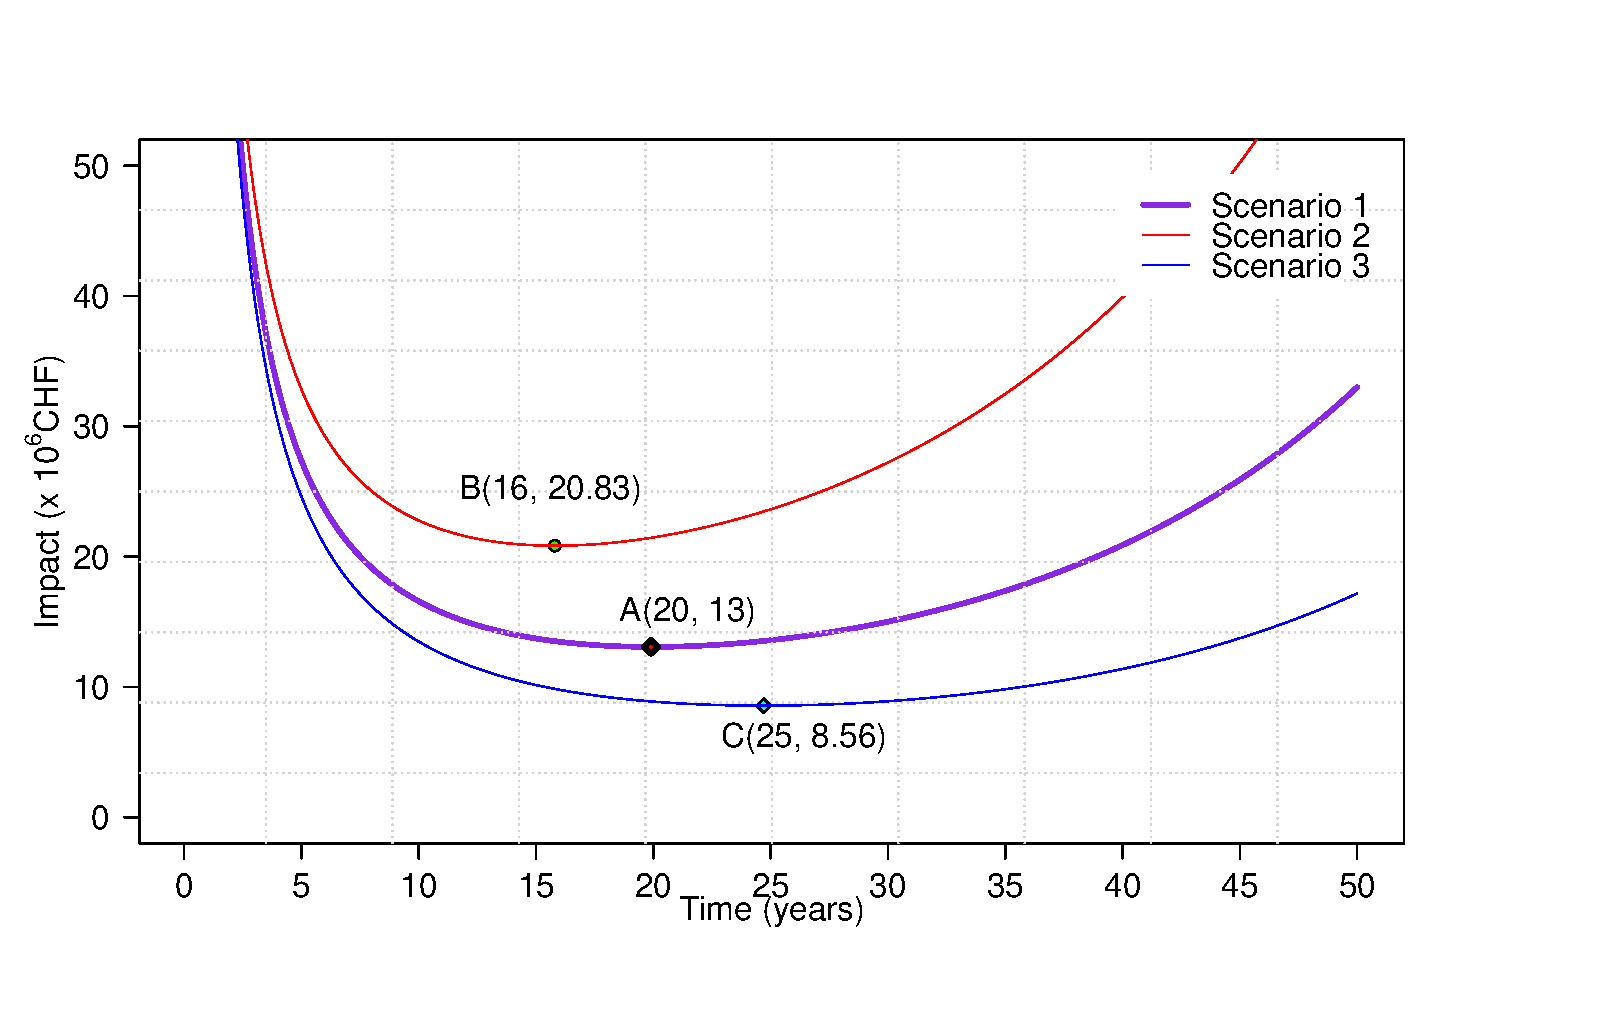
\includegraphics[scale=0.4]{fig2} 	
\end{center}
\caption{Deterioration Expectation Path.}
\label{fig2}
\end{figure}

 \begin{table}
      \begin{center}
         \caption{Sample Mean of the Markov Transition Probability based on the Bayesian Estimation (Data set $D_{2000}$ used)}
         \label{table5}
         {\small
   \begin{tabular}{c|ccccccc|c}
\hline
Condition states & 1 & 2 & 3 & 4 & 5 & 6 & 7 & Hazard rate \\ 
\hline
 1 & 0.7649 & 0.2046 &0.0285 & 0.0019 & 0.0000 & 0.0000 & 0.0000 & 0.2680 \\
   2 & 0 & 0.7618 & 0.2154 & 0.0220 & 0.0008 & 0.0000 & 0.0000 & 0.2720 \\
   3 & 0 & 0 & 0.8229 & 0.1682 & 0.0086 & 0.0003 & 0.0000 &0.1949 \\
   4 & 0 & 0 & 0 & 0.9045 & 0.0907 & 0.0046 & 0.0002 &0.1004 \\
   5 & 0 &0 &0 &0 & 0.9032 & 0.0908 & 0.0060 &0.1018 \\
   6 & 0 &0 &0 &0 &0 & 0.8811 &  0.1189 &0.1266 \\
   7 & 0 &0 &0 &0 &0 &0 &1 &- \\ 
   \hline
\end{tabular}     
         }
      \end{center}
\end{table}


\begin{table}
      \begin{center}
         \caption{Markov Transition Probability based on the MLE Method (Original database used)}
         \label{table6}
         {\small
   \begin{tabular}{c|ccccccc|c}
\hline
Condition states & 1 & 2 & 3 & 4 & 5 & 6 & 7 & Hazard rate \\ 
\hline
1 & 0.6862 & 0.2749 &0.0368 & 0.0021 & 0.0001 & 0.0000 & 0.0000 & 0.3766 \\
   2 & 0 & 0.7756 & 0.2064 & 0.0174 & 0.0006 & 0.0000 & 0.0000 & 0.2541 \\
   3 & 0 & 0 & 0.8497 & 0.1422 & 0.0078 & 0.0002 & 0.0000 &0.1628 \\
   4 & 0 & 0 & 0 & 0.8977 & 0.0974 & 0.0046 & 0.0003 &0.1079 \\
   5 & 0 &0 &0 &0 & 0.9067 & 0.0844 & 0.0089 &0.0980 \\
   6 & 0 &0 &0 &0 &0 & 0.8174 &  0.1826 &0.2017 \\
   7 & 0 &0 &0 &0 &0 &0 &1 &- \\
      \hline
\end{tabular}     
         }
      \end{center}
\end{table}



\subsubsection*{b) Condition state distribution}
In order to grasp the average deterioration states of structures or specific members, it is effective to calculate the deterioration expectation path. On the other hand, it would also be important to grasp the time-series variation of the condition state distribution of the entire set of structures or the entire set of members, for carrying out asset management. Then, using the Markov transition probability, the time-series variation of the condition state distribution is analyzed.

If the hazard rate of the Gibbs sample $n$ defined by Eq. (\ref{wuei}) based on the Bayesian estimation is obtained, the Markov transition probability can be estimated from Eqs.(\ref{pj}) and (\ref{1pj}). Furthermore, as in the case of the expected condition state duration, the sample mean $E[p_{ij}(n:\bar{\mbox{\boldmath$x$}}^k)]$ and sample order statistic $(\underline{p}^{\alpha}_{ij}(\bar{\mbox{\boldmath$x$}}^k),\overline{p}^{\alpha}_{ij}(\bar{\mbox{\boldmath$x$}}^k))$ of the Markov transition probability of the inspection sample $k$ are defined. The definition of the concrete equation is omitted; refer to Eqs. (\ref{sampmean}), (\ref{conf1}), and (\ref{conf2}), if necessary. Table \ref{table5} shows the sample mean $E[p_{ij}(n:\bar{\mbox{\boldmath$x$}}^k)]$ of the Markov transition probability calculated from the results of the Bayesian estimation of $D_{2000}$, and Table \ref{table6} shows the Markov transition probability calculated from the maximum-likelihood estimate. As for the Markov transition probability, it is possible to evaluate the confidence interval by calculating the sample order statistics.

Next, the condition state distribution is calculated. Consider the case in which all RC slabs in N city are new at timing $t$. The condition states are all $1$, and so the initial value of the state vector is defined as $\mbox{\boldmath$X$}_{t}=(1,0,0,0,0,0,0)$. The arbitrary timing $t$ was specified as $t=0$ and the calculation was repeated 100 times. Since the inspection interval of the estimated Markov transition probability is one year, by repeating the calculation 100 times, it is possible to grasp the $100$ years condition state distribution. 

Fig. \ref{fig3} shows the transition of the condition state distribution when the Markov transition probability (in Table \ref{table6}) that has been estimated from $D_{2000}$ is used. There are few RC slabs whose condition state is still $1$ at $20$ years later. After that, deterioration progresses, and the occupancy rates of higher condition states (which indicate the progress of deterioration) increase. In addition, it can be understood that around 40 years after the start of deterioration, where the sample mean of the expected condition state duration is provided by the deterioration expectation path in the previous section, about 50$\%$ of RC slabs have reached the condition state $i=7$. In addition, based on the 90$\%$ confidence lower-limit and upper-limit values $(\underline{p}^{\alpha}_{ij}(\bar{\mbox{\boldmath$x$}}^k),\overline{p}^{\alpha}_{ij}(\bar{\mbox{\boldmath$x$}}^k))$ of the Markov transition probability, pessimistic and optimistic scenarios can be calculated respectively.
%

\begin{figure}[t]
\begin{center}
\includegraphics[scale=0.5]{fig3} 
\end{center}
\caption{Condition state distribution, sample mean of the Markov transition probability $E[p_{ij}(n:\bar{\mbox{\boldmath$x$}}^k)]$.}
\label{fig3}
\end{figure}

\section{Conclusion}\label{section6}
This study focuses on a case in which condition state is evaluated with multi-state condition state incorporating visual inspection results, and proposes a methodology for conducting the Bayesian estimation of the Markov transition probability, using the multi-state Markov model. When the accumulation of the inspection data regarding the deterioration state of civil infrastructures is not enough, there is no choice but to estimate a deterioration prediction model, by utilizing the information based on the experience of professional engineers and the estimation results at structures in other regions. 

The Bayesian estimation has a preferable feature: it is possible to utilize the prior experience-based information of engineers as prior information and combine it with actual measurement data based on visual inspection results and then predict deterioration. In addition, this study discussed empirically the effectiveness of the Bayesian estimation of the multi-state Markov  model, using the results of the visual inspection of the RC slabs of the bridges maintained by N city. The results indicate that when accurate prior information is provided, it is possible to obtain estimation results whose precision is at the same level as in the MLE method, based on a plentiful amount of inspection samples, even if the amount of visual inspection samples is small. The methodology of conducting the Bayesian estimation of the multi-state Markov model can be considered to be excellent in the flexibility and extendibility of the model and highly practical and it is possible to apply this methodology to the deterioration prediction for a variety of civil infrastructures, by accumulating data.

On the other hand, with regard to the development of a statistical deterioration prediction method based on visual inspection data, the following issues remain to be studied in the future. The first is the Bayesian estimation of time-dependent deterioration processes. The second is the Bayesian estimation for the case in which there is some bias in the sampling data. That is, there emerges the problem of sample shortage: when deterioration has progressed, some countermeasure is conducted, and so the amount of inspection samples regarding the condition states decreases. The third is the deterioration prediction of individual structures or individual members. Each civil infrastructure sometimes has heterogeneity that cannot be ignored. The fourth is the deterioration prediction that takes into account the effects of error in visual inspection results.

\section{Acknowledgment}
This study was financially supported by Special Coordination Funds for Promoting Science and Technology, Ministry of Education, Culture, Sports, Science and Technology, Japan. The authors would like to thank the Frontier Research Base for Global Young Researchers, Graduate School of Engineering, Osaka University, where a part of this study was conducted.
\bibliographystyle{ascelike}
\bibliography{reference}
\end{document}